
\documentclass[12pt]{article}

\usepackage[margin=1in]{geometry}
\usepackage{amsmath,amssymb,booktabs,array}
\usepackage{enumitem}
\usepackage{setspace}
\usepackage{graphicx}
\usepackage{caption}
\usepackage{hyperref}

\graphicspath{{figures/}}
\captionsetup{font=small,labelfont=bf}

\hypersetup{
    colorlinks=true,
    linkcolor=black,
    urlcolor=black
}

\onehalfspacing
\setlength{\parindent}{2.75em}
\setlist[enumerate,1]{leftmargin=*,itemsep=1.5ex}
\setlist[enumerate,2]{leftmargin=*,itemsep=1ex}

\begin{document}

\begin{center}
\large{\textbf{ECON 344: Economics of Crime \\
TA Section: The Economic Costs of Gender-Based Violence}}
\end{center}

\medskip

\noindent\textbf{Content Note:}
This handout discusses sexual assault, gender-based violence,
and workplace harassment. We recognize that these topics
may be difficult or sensitive for some students.
All questions concern research methods, economic mechanisms,
and hypothetical examples. No one will be asked to share
personal experiences. Students may step away or skip a question
without needing to explain why.

\bigskip

% ============================================================
\section*{Question 1: The Economic Consequences of Sexual Assault}
% ============================================================

\noindent\textit{Reference:}
Adams, Abi, Kristiina Huttunen, Emily Nix, and Ning Zhang
(2026). ``The Economic Impacts of Sexual Assault.''
Institute for Fiscal Studies, Working Paper W26/15.

\medskip

\noindent\textbf{Study:}
Adams et al. (2026) use Finnish administrative records,
including police reports, hospital admissions, and
longitudinal economic records, to study the consequences
of sexual assault.

The authors compare survivors to observationally similar
women who did not experience a recorded assault.
They find that, over the five years following an assault,
employment falls by approximately 6 percentage points
and annual earnings decline by approximately 1,500 euros.
They also document increases in antidepressant use,
persistent effects over time, and mental health spillovers
to family members and female schoolmates.

\begin{enumerate}

\item \textbf{Identifying the economic costs of violence.}

Suppose a researcher compares the earnings of women
who have experienced sexual assault to those who have not
and finds that survivors earn less.

\begin{enumerate}

\item Why would this comparison not necessarily identify
the causal effect of sexual assault on earnings?

% SOLUTION:
% Women experiencing assault may differ from other women
% in prior economic circumstances, neighborhoods,
% employment histories, or other characteristics.
% These differences may independently predict earnings.
% Thus, a cross-sectional earnings gap combines the
% consequences of assault with pre-existing differences.
\vspace{4cm}

\item Suppose the researcher observes earnings for several
years before and after the assault. How could these data
help construct a more credible comparison?
What identifying assumption would still be necessary?

% SOLUTION:
% The researcher could compare changes in earnings among
% survivors with changes among observationally similar
% women who do not experience a recorded assault.
% A causal interpretation requires that the groups'
% potential earnings would have followed parallel trends
% in the absence of the assault, conditional on controls.
% Similar pre-trends are reassuring but not sufficient.
\vspace{4cm}

\end{enumerate}

\vspace{1cm}

\item \textbf{Writing an event-study regression.}

Let $Y_{it}$ denote annual earnings for woman $i$
in year $t$. Let $D_i=1$ for women who experience
a recorded assault, and let $k$ denote years relative
to the event, with $k=0$ in the year of the assault.

\begin{enumerate}

\item Write an event-study regression that includes
individual fixed effects, calendar-year fixed effects,
and interactions between $D_i$ and indicators for
event time. Use $k=-1$ as the omitted reference period.

% SOLUTION:
% One possible specification is:
%
% Y_it = alpha_i + lambda_t
%        + sum_{k != -1} beta_k
%          [D_i x 1{event time_it = k}]
%        + epsilon_it.
%
% alpha_i represents individual fixed effects.
% lambda_t represents calendar-year fixed effects.
% beta_k is the treated-control difference at event
% time k relative to the omitted pre-event period.
%
% In an actual matched staggered-event design, one
% must define event time for comparison women and
% account for possible heterogeneous treatment effects.
\vspace{4cm}

\item What does $\beta_3$ represent?
What would you expect the coefficients for
$k<0$ to look like if the design is credible?

% SOLUTION:
% beta_3 measures the relative change in earnings
% three years after the event compared with the
% treated-control difference one year before it.
% Pre-event coefficients should be close to zero
% without a systematic trend if the groups have
% similar pre-treatment trajectories.
% This does not establish parallel trends definitively.
\vspace{4cm}

\item Suppose the estimated coefficient three years
after the assault is $-1500$, with a standard error
of $500$. Interpret the coefficient and determine
whether it is statistically significant at the
5\% level.

% SOLUTION:
% The estimate implies a 1,500 euro reduction in
% annual earnings three years after the assault,
% relative to the comparison group's counterfactual
% trend, under the identifying assumptions.
%
% The t-statistic is -1500/500 = -3.
% The approximate 95% confidence interval is
% [-2480, -520], excluding zero.
% Thus the estimate is statistically significant
% at the 5% level.
%
% These numerical coefficient and SE values are
% hypothetical for the exercise.
\vspace{4cm}

\end{enumerate}

\vspace{1cm}

\item \textbf{Reading the event-study results.}

Figure~\ref{fig:adams-labor} reproduces the paper's main
labor market results. Panel I plots raw means for survivors
and matched control women. Panel II plots the event-study
coefficients $\hat\beta_k$ with 95\% confidence intervals,
normalized to zero at $k=-1$.

\begin{center}
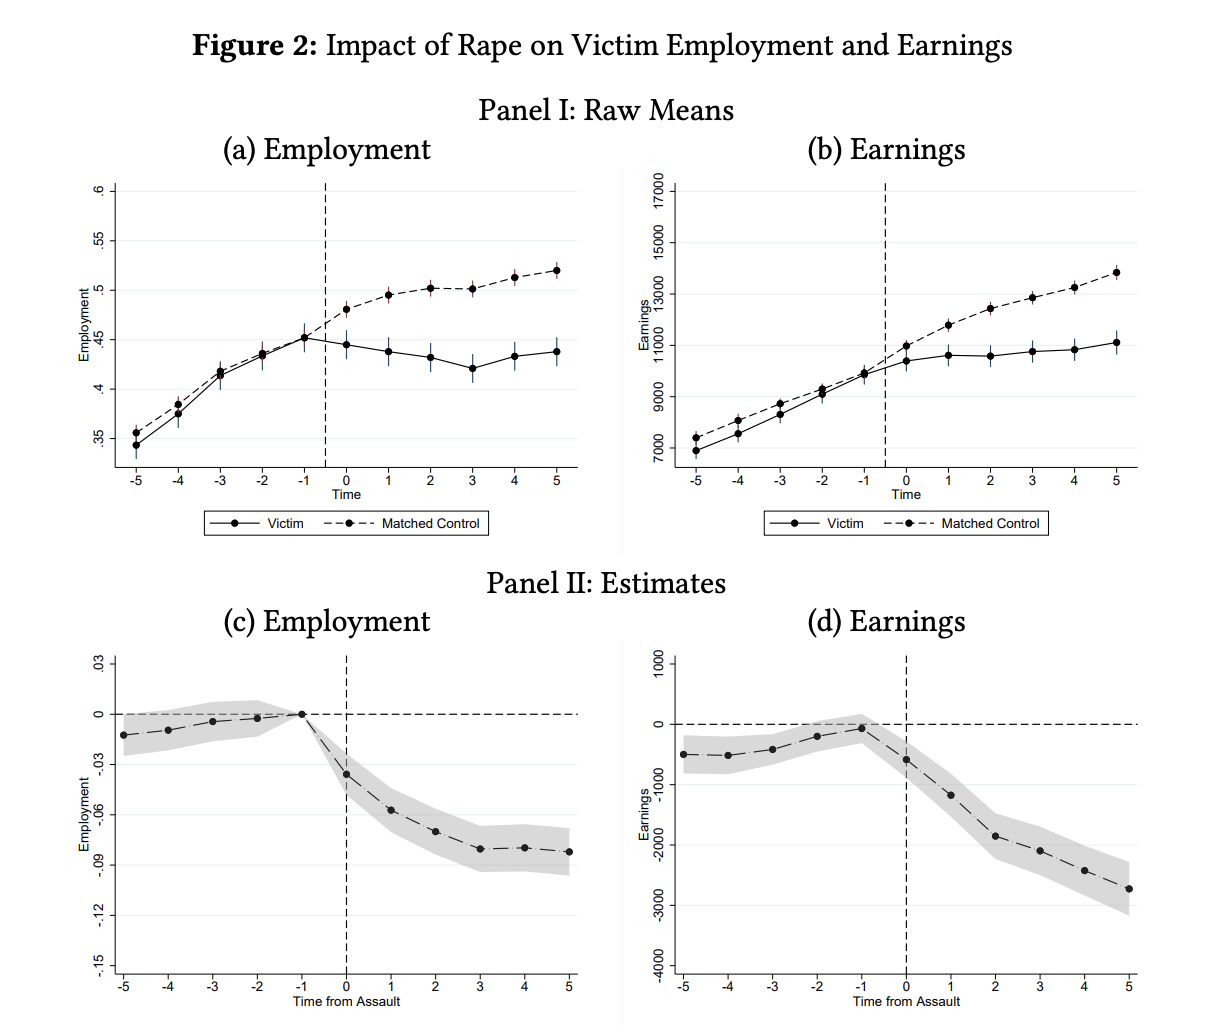
\includegraphics[width=0.95\textwidth]{adams2026_employment_earnings.png}
\captionof{figure}{Employment and earnings around the assault.
Source: Adams et al.\ (2026), Figure 2.}
\label{fig:adams-labor}
\end{center}

\begin{enumerate}

\item In Panel I, survivors' earnings continue to rise
after $k=0$ and their employment roughly flattens rather
than collapsing, yet Panel II shows large negative effects. Explain how both can be true.
What does the matched control group contribute here
that a simple before--after comparison of survivors
would not?

% SOLUTION:
% Both groups are young women whose employment and
% earnings are rising with age and labor market entry.
% A before-after comparison of survivors alone would
% attribute that life-cycle growth to the post period
% and could even suggest assault has no effect or a
% positive one. The matched controls show what the
% survivors' trajectory would plausibly have been;
% the effect is the gap that opens up between the
% two lines after k = 0, which is what Panel II plots.
\vspace{4cm}

\item Use Panel II to describe the \emph{dynamics}
of the effects. Roughly how large is the employment
effect at $k=0$ and at $k=5$? Is the earnings loss
temporary or persistent?

% SOLUTION:
% Employment falls by about 3-4 percentage points in
% the year of the assault and continues to decline,
% reaching roughly 8 percentage points by k = 3, where
% it levels off. Earnings losses grow steadily, from
% about 600 euros at k = 0 to roughly 2,700 euros at
% k = 5, with no sign of recovery. The effects are
% persistent and, for earnings, still widening.
% (Students should read approximate magnitudes off
% the figure; exact values are not required.)
\vspace{4cm}

\item Look at the pre-period coefficients ($k<-1$).
Are they exactly zero? Suppose the pre-period pattern
reflects a true pre-existing trend that would have
continued. Would the post-period estimates then
overstate or understate the true effect of assault?

% SOLUTION:
% They are not exactly zero: survivors start slightly
% below controls (about -0.01 in employment and -500
% euros in earnings at k = -5) and close the gap by
% k = -1, i.e. survivors were catching up before the
% assault. The confidence intervals mostly include
% zero for employment.
% If that convergence would have continued, the true
% counterfactual for survivors lies ABOVE the zero
% line after k = 0, so the estimated declines would
% UNDERSTATE the true effect (the estimates are
% conservative). This is a reminder that "no
% significant pre-trends" is evidence, not proof,
% of parallel trends.
\vspace{4cm}

% \item Compare the magnitudes in Panel II with the
% hypothetical coefficient in part 2(c). Why is it
% important to state the time horizon when reporting
% the ``effect'' of an event with dynamic impacts?

% SOLUTION:
% The figure shows earnings effects of roughly
% -2,100 euros at k = 3, larger than the hypothetical
% -1,500. More generally, because effects grow over
% time, a single number (e.g. "1,500 euros") can
% refer to an average over years 0-5, an effect at a
% particular horizon, or a cumulative loss. These can
% differ by a lot; cumulative losses over five years
% are several times larger than any one-year effect.
\vspace{4cm}

\end{enumerate}

\vspace{1cm}

\item \textbf{Mental health and household outcomes.}

Figure~\ref{fig:adams-mech} shows event-study estimates
for two non-labor-market outcomes: an indicator for
antidepressant use and an indicator for cohabiting with
a partner.

\begin{center}
\noindent\begin{minipage}{0.48\textwidth}
\centering
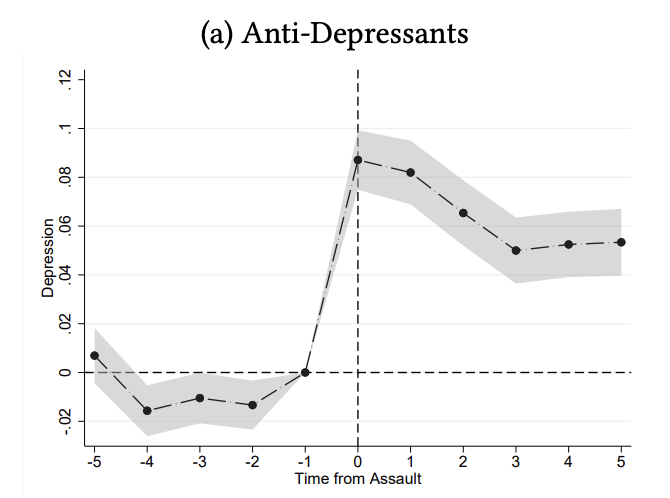
\includegraphics[width=\textwidth]{adams2026_antidepressants.png}
\end{minipage}\hfill
\begin{minipage}{0.48\textwidth}
\centering
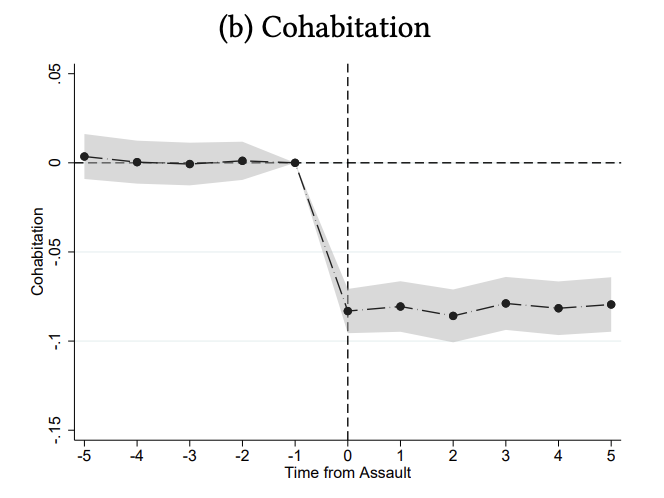
\includegraphics[width=\textwidth]{adams2026_cohabitation.png}
\end{minipage}
\captionof{figure}{Antidepressant use and cohabitation around the
assault. Source: Adams et al.\ (2026).}
\label{fig:adams-mech}
\end{center}

\begin{enumerate}

\item Compare the \emph{timing} of the antidepressant
effect with the timing of the employment effect in
Figure~\ref{fig:adams-labor}. How might this pattern
help us think about mechanisms linking assault to
labor market outcomes? Does it prove that mental
health is the mechanism?

% SOLUTION:
% Antidepressant use jumps immediately, by about 9
% percentage points at k = 0, then partially fades
% to a persistent ~5 pp increase. Employment, by
% contrast, declines gradually over several years.
% A mental health shock that precedes and persists
% alongside labor market losses is consistent with
% mental health being one channel through which
% assault reduces employment and earnings.
% It does not prove it: assault may affect earnings
% through other channels at the same time (physical
% injury, changes in household structure, leaving a
% job where the perpetrator works, legal proceedings),
% and antidepressant use is itself an outcome of the
% assault, not randomly assigned.
\vspace{4cm}

\item Cohabitation falls by about 8 percentage points
in the year of the assault and does not recover.
Give two different explanations for this pattern.
Why might this matter for interpreting the earnings
results?

% SOLUTION:
% (1) In some cases the perpetrator may be a partner,
% so separation is a direct consequence of (or
% response to) the violence. (2) The trauma of an
% assault by someone else may strain existing
% relationships or delay new ones.
% This matters because household dissolution can
% itself affect labor supply and financial security
% (e.g. losing a partner's income may push some women
% into work, or relocation may disrupt employment).
% The earnings effects therefore combine the direct
% effect of the assault with effects operating
% through changes in household structure. Separating
% these would require analyzing subgroups (e.g. by
% relationship to the perpetrator), not simply
% controlling for cohabitation, which is a "bad
% control" since it is affected by the treatment.
\vspace{4cm}

\item The antidepressant pre-period coefficients at
$k=-4$ to $k=-2$ are slightly negative and some
confidence intervals exclude zero. Does this
invalidate the design?

% SOLUTION:
% Not necessarily. The pre-period estimates are small
% (about -1.5 pp) relative to the post-period jump
% (about +9 pp), and there is no steady trend that
% could mechanically generate the sharp break at
% k = 0. One would want to check robustness to
% alternative control groups or matching variables,
% whether the pattern reflects a few cohorts, and how
% sensitive the estimates are to allowing for a
% linear pre-trend (e.g. Rambachan-Roth style bounds).
\vspace{4cm}

\end{enumerate}

\vspace{1cm}

\clearpage
\item \textbf{Selection into reporting.}

Administrative records do not capture every sexual
assault. Some survivors report incidents to police,
some seek medical attention, and others do neither.

\begin{enumerate}

\item Suppose more economically disadvantaged survivors
are less likely to report an assault.
Why could this affect the interpretation of the
study's estimates? Would the direction of bias
necessarily be known?

% SOLUTION:
% The observed sample of recorded assaults may not
% represent all survivors. If reporting is correlated
% with socioeconomic status and treatment effects,
% estimates may not generalize to unreported assaults.
% The direction of bias is ambiguous because reporting
% may be associated with either more or less severe
% economic consequences, conditional on other factors.
\vspace{4cm}

% \item Suppose an outreach program increases reporting
% without changing the actual incidence of sexual assault.
% What happens to the number of recorded incidents?
% Why does this distinction matter when evaluating policy?

% SOLUTION:
% Recorded incidents may increase even though true
% incidence remains unchanged.
% Thus, an increase in police reports does not
% necessarily imply an increase in actual violence.
% Reporting behavior must be distinguished from
% the underlying incidence of violence.
\vspace{4cm}

\end{enumerate}

\vspace{1cm}

\item \textbf{Spillovers and total economic costs.}

The authors also find evidence of mental health
consequences among family members and schoolmates
of survivors.

\begin{enumerate}

\item Explain why estimating earnings losses only
among survivors might understate the total social
costs of sexual assault.

% SOLUTION:
% Costs can extend beyond the direct survivor through
% effects on family members, peers, workplaces,
% healthcare expenditures, and well-being.
% These costs would not be included in estimates
% based only on survivors' earnings losses.
\vspace{4cm}

\item Suppose a government calculates the benefits
of a prevention program using only earnings losses
averted among survivors.
Would this necessarily overstate or understate the
social benefits of prevention? Explain.

% SOLUTION:
% It would generally omit other benefits of preventing
% violence, such as improvements in physical and mental
% health and reduced spillovers to other people.
% Hence it is likely to understate total benefits,
% assuming the omitted consequences are social costs.
% However, a complete welfare calculation must avoid
% double counting overlapping consequences.
\vspace{4cm}

\end{enumerate}

\end{enumerate}


\clearpage

% ============================================================
\section*{Question 2: Street Harassment and Educational Choices}
% ============================================================

\noindent\textit{Reference:}
Borker, Girija (2021).
``Safety First: Perceived Risk of Street Harassment
and Educational Choices of Women.''

\medskip

\noindent\textbf{Study:}
Borker (2021) studies how concerns about street harassment
affect college choices among students at the University
of Delhi, India.

The author combines student survey data, information on
college quality, potential commuting routes to colleges
in each student's choice set, and crowdsourced data on
the perceived safety of different locations.

Using a model of college choice, the paper estimates how
students trade off college quality, commuting costs,
travel time, and safety. Because students respond to
perceived risk, the threat of harassment can impose
economic costs even when no incident is observed.

\begin{enumerate}

\item \textbf{Identifying the costs of unsafe public spaces.}

Suppose we observe that female students attend lower-ranked
colleges than male students, on average.

\begin{enumerate}

\item Why would this difference not necessarily identify
the effect of street harassment on women's college choices?
Give one specific alternative explanation.

% SOLUTION:
% Men and women may differ in admission scores, financial
% resources, home locations, preferences, and available
% colleges. These differences could generate different
% college choices even in the absence of harassment.
% Therefore, the observed gender gap is not necessarily
% caused by differences in perceived safety.
\vspace{4cm}

\item Why is it important that Borker observes the colleges
students could have attended, including those they did
not choose? Why does she also construct potential
commuting routes to these colleges?

% SOLUTION:
% A student's decision depends on the feasible alternatives.
% College quality, travel time, cost, and safety differ
% across these alternatives.
% Observing only the chosen college cannot reveal
% which tradeoffs the student faced.
% Constructing potential routes lets the researcher
% compare the safety and commuting costs of chosen
% versus unchosen alternatives.
\vspace{4cm}

\end{enumerate}

\vspace{1cm}

\item \textbf{The economics of safety and educational choice.}

Consider a student choosing between two colleges:

\begin{center}
\begin{tabular}{lcc}
\toprule
& College A & College B \\
\midrule
College quality index & 90 & 75 \\
Commute time (minutes) & 45 & 30 \\
Perceived safety index & 4 & 8 \\
\bottomrule
\end{tabular}
\end{center}

Higher values indicate better college quality
and greater perceived safety.

\begin{enumerate}

\item Why might a student choose College B even though
College A has higher academic quality?
Explain using the concept of utility maximization.

% SOLUTION:
% Students maximize utility rather than academic
% quality alone. A student may prefer College B
% because its commute is shorter and safer.
% The additional safety and time savings may outweigh
% the educational benefits of College A.
% Such a decision need not be irrational.
\vspace{4cm}

\item Suppose the student's utility from attending
college $j$ is:

\[
U_{ij}
=
\beta_Q Q_j
+
\beta_S S_{ij}
-
\beta_T T_{ij}
+
\varepsilon_{ij},
\]

where $Q_j$ is college quality, $S_{ij}$ is perceived
route safety, and $T_{ij}$ is commuting time.

Assume $\beta_Q,\beta_S,\beta_T>0$.
Derive the condition under which the student
prefers College B to College A.

% SOLUTION:
% U_iB - U_iA =
% beta_Q(75-90) + beta_S(8-4)
% - beta_T(30-45) + epsilon_iB-epsilon_iA.
%
% College B is preferred if:
% 4 beta_S + 15 beta_T
% + epsilon_iB-epsilon_iA > 15 beta_Q.
%
% Safety and travel-time benefits must outweigh
% the loss of college quality, adjusted for other
% unobserved preferences.
\vspace{4cm}

\item Suppose $\beta_Q=1$, $\beta_S=3$,
$\beta_T=0.2$, and the unobserved utilities
are equal across the two colleges.
Which college would the student choose?

% SOLUTION:
% College A utility:
% 90 + 3(4) - 0.2(45) = 93.
%
% College B utility:
% 75 + 3(8) - 0.2(30) = 93.
%
% The student is indifferent between the colleges.
% If beta_S increases, College B becomes preferred.
% If beta_Q increases, College A becomes preferred.
\vspace{4cm}

\end{enumerate}

\vspace{1cm}

\item \textbf{Estimating preferences for safety.}

Now add travel expenditure to the model. Consider a
simplified version of the college-choice model used
in the paper:

\[
U_{ij} =
\beta_Q Q_j
+\beta_S S_{ij}
-\beta_C C_{ij}
-\beta_T T_{ij}
+\varepsilon_{ij},
\]

where $Q_j$ is college quality, $S_{ij}$ is the perceived
safety of the commute, $C_{ij}$ is annual travel
expenditure (in rupees), and $T_{ij}$ is travel time.

Assume all four coefficients are positive.

\begin{enumerate}

\item Suppose a safer commuting route improves safety by
one unit but requires an additional annual expenditure
of $c$ rupees. Holding everything else constant, derive
the maximum amount the student would be willing to pay
for the safer route.

% SOLUTION:
% Holding utility constant:
% beta_S(1) - beta_C(c) = 0.
%
% Therefore, c = beta_S / beta_C.
% This is the willingness to pay for a one-unit
% improvement in perceived commuting safety.
\vspace{4cm}

\vspace{4cm}

\item Why might the ratio $\beta_S/\beta_C$ differ
between female and male students? What would a larger
ratio for women imply about the economic costs of
street harassment?

% SOLUTION:
% Women may face greater actual or perceived risks
% of street harassment during their commutes.
% A higher ratio means women are willing to sacrifice
% more money to obtain the same improvement in safety.
% This reveals an additional cost of unsafe public
% spaces borne disproportionately by women.
% Differences could also reflect other gender-specific
% preferences or constraints.
\vspace{4cm}


\end{enumerate}

\vspace{1cm}

\item \textbf{Interpreting the paper's results.}

Borker finds that, for a route perceived to be one
standard deviation safer, women are willing to choose
a college in the bottom half of the quality distribution
instead of one in the top 20 percent.

Men are willing to make a much smaller sacrifice in
college quality for the same safety improvement.

The paper also estimates that women are willing to
spend approximately INR 17,500 per year for a route
perceived to be one standard deviation safer, compared
with approximately INR 9,950 for men.

\begin{enumerate}

\item What do these findings suggest about the relationship
between perceived safety and women's human capital
investment? Explain why choosing a lower-ranked college
does not necessarily imply that a student is making
an irrational decision.

% SOLUTION:
% Unsafe commuting routes may lead women to sacrifice
% educational quality to reduce their exposure to
% perceived harassment risk.
% This can reduce human capital accumulation and
% potentially future earnings.
% However, choosing the safer college can be fully
% rational given the student's preferences, risks,
% and available alternatives.
\vspace{4cm}

\item Calculate the difference between women's and men's
annual willingness to pay for a one-standard-deviation
improvement in safety. Why might this difference be
informative about the gender-specific costs of unsafe
public spaces?

% SOLUTION:
% 17,500 - 9,950 = INR 7,550 per year.
%
% Women's estimated willingness to pay is about
% 76% higher than men's:
% (17,500 / 9,950 - 1) x 100 = 75.9%.
%
% The gender difference is informative about the
% additional value women place on commuting safety.
% It does not necessarily equal the direct monetary
% cost of harassment, because safety perceptions
% and other constraints may also differ by gender.
\vspace{4cm}

\item The paper's sample consists of students who enrolled
at the University of Delhi. Would these estimates
necessarily capture the full economic costs of unsafe
commuting for all young women in Delhi? Explain.

% SOLUTION:
% No. The sample excludes women who did not enroll
% in college, potentially because commuting risks
% made attendance too costly.
% The estimates therefore capture tradeoffs among
% enrolled students but not the extensive-margin
% decision to attend college at all.
% They may understate the broader educational costs
% of unsafe public spaces.
\vspace{4cm}

\end{enumerate}

\vspace{1cm}


\item \textbf{Policy implications.}

A policymaker concludes:
``If women choose lower-quality colleges because of
unsafe commutes, the government should simply give
female students more money for transportation.''

Would transportation subsidies necessarily eliminate
the educational costs identified in Borker (2021)?
Explain how the effectiveness of this policy depends
on the mechanism driving women's choices.

% SOLUTION:
% Not necessarily. A subsidy may help if safer travel
% options exist but are too expensive for students.
% However, if all feasible routes involve substantial
% harassment risk, lower transportation costs alone
% may not solve the underlying safety problem.
% Investments in safer transport, public-space safety,
% and enforcement might be necessary.
% The preferred policy depends on whether money,
% travel time, or the lack of safe alternatives
% is the binding constraint.
\vspace{4cm}

\end{enumerate}


\clearpage

% ============================================================
\section*{Question 3: Violence Against Women at Work}
% ============================================================

\noindent\textit{Reference:}
Adams, Abi, Kristiina Huttunen, Emily Nix, and Ning Zhang
(2024). ``Violence Against Women at Work.''
\emph{Quarterly Journal of Economics}.

\medskip

\noindent\textbf{Study:}
Adams et al. (2024) link Finnish police reports
to administrative employment records to study
violence between coworkers.

They find persistent labor market consequences
for victims of workplace violence, while men who
assault female colleagues face weaker consequences
than men who assault male colleagues.

The authors also find that violence against female
coworkers is followed by declines in women's
representation at affected firms, reflecting both
lower hiring and increased departures.

Importantly, these workforce changes are concentrated
in male-managed firms.

\begin{enumerate}

\item \textbf{Individual versus firm-level costs.}

Suppose a female employee experiences an assault
by a male coworker. Following the incident,
she leaves the firm and begins working elsewhere
at a lower wage.

\begin{enumerate}

\item Identify two distinct economic costs of the
incident for the employee.

% SOLUTION:
% Possible costs include reduced earnings,
% loss of firm-specific human capital,
% unemployment or job-search costs,
% career disruption, and deterioration
% in physical or mental health.
% Some costs are monetary while others are
% nonmonetary.
\vspace{4cm}

\item Could the incident also affect employees
who were not directly involved?
Give one possible economic mechanism.

% SOLUTION:
% Other employees may perceive the workplace
% as less safe, resulting in lower productivity,
% increased turnover, or reluctance to accept
% employment at the firm.
% Such spillovers mean the cost to the firm
% and its workers can exceed the direct
% costs experienced by the survivor.
\vspace{4cm}

\end{enumerate}

\vspace{1cm}

\item \textbf{Difference-in-differences.}

Suppose a researcher studies the share of employees
who are women at firms where an assault against
a female coworker is recorded.

The researcher compares these firms to otherwise
similar firms without a recorded incident.

Consider the following \textbf{hypothetical} data:

\begin{center}
\begin{tabular}{lcc}
\toprule
& Before & After \\
\midrule
Firms with recorded incident & 0.45 & 0.39 \\
Comparison firms & 0.43 & 0.42 \\
\bottomrule
\end{tabular}
\end{center}

\begin{enumerate}

\item Calculate the difference-in-differences
estimate of the effect of a recorded workplace
violence incident on the female employment share.
Interpret its units.

% SOLUTION:
% Treated firms: 0.39 - 0.45 = -0.06.
% Comparison firms: 0.42 - 0.43 = -0.01.
% DiD = -0.06 - (-0.01) = -0.05.
%
% The estimated effect is a 5 percentage point
% decline in the female employment share,
% relative to the comparison firms,
% under the identifying assumptions.
\vspace{4cm}

\item Let $Y_{ft}$ denote the female employment
share in firm $f$ at time $t$.
Write a difference-in-differences regression
with firm fixed effects, time fixed effects,
and a treatment-by-post interaction.

Which coefficient captures the causal
effect of the incident?

% SOLUTION:
% Y_ft = alpha_f + lambda_t
%        + beta(Treated_f x Post_t)
%        + epsilon_ft.
%
% alpha_f captures time-invariant firm characteristics.
% lambda_t captures shocks common to all firms.
% beta is the DiD estimate, interpreted causally
% under parallel trends and other assumptions.
\vspace{4cm}

\item State the identifying assumption.
Give one plausible example of how it could
be violated in this setting.

% SOLUTION:
% In the absence of the incident, treated
% and comparison firms would have experienced
% similar changes in female employment shares.
%
% For example, a firm experiencing worsening
% management conditions might simultaneously
% experience increased workplace violence
% and declining female employment.
% This would violate parallel trends if
% comparison firms did not experience the
% same deterioration.
\vspace{4cm}

\end{enumerate}

\vspace{1cm}

\item \textbf{Gender, management, and mechanisms.}

The authors find that male perpetrators experience
weaker labor market consequences after assaulting
female colleagues than after assaulting male colleagues.
They also find different firm-level outcomes depending
on whether firms have male or female managers.

\begin{enumerate}

\item Suggest one economic mechanism that could
explain why perpetrator consequences differ
depending on the gender of the victim.

% SOLUTION:
% Differences may reflect relative bargaining
% power, economic dependence on the perpetrator,
% managerial incentives, or differential sanctions.
% For example, employers may be more reluctant
% to dismiss economically valuable perpetrators,
% allowing the costs to fall disproportionately
% on female victims.
% Differences in incident characteristics could
% also contribute and must be addressed empirically.
\vspace{4cm}

\item Suppose female-managed firms exhibit
smaller declines in female employment after
a recorded incident than male-managed firms.

Can we conclude that appointing a female manager
would causally reduce the employment consequences
of workplace violence? Explain.

% SOLUTION:
% No. Manager gender is not randomly assigned.
% Male- and female-managed firms may differ in
% workplace culture, employee composition,
% reporting procedures, and other characteristics.
% The observed heterogeneity is consistent
% with management playing a role, but does not
% by itself identify the causal effect of
% appointing a female manager.
\vspace{4cm}

\item What additional evidence would strengthen
the hypothesis that managerial responses
explain the differences between firms?

% SOLUTION:
% Researchers could investigate perpetrator
% retention, disciplinary actions, worker exits,
% and hiring changes following incidents.
% Evidence from plausibly exogenous changes
% in management could strengthen causal claims.
% Observing stronger sanctions against perpetrators
% and smaller female workforce losses would
% support the proposed mechanism, although
% the analysis must address selection.
\vspace{4cm}

\end{enumerate}

\vspace{1cm}

\clearpage
\item \textbf{An important measurement concern.}

Suppose firms with stronger reporting procedures
are more likely to have workplace violence
recorded by authorities, even if their actual
incidence of violence is no higher.

How might this affect a comparison between
firms with and without recorded incidents?
What additional information could help
address this concern?

% SOLUTION:
% Recorded incidents may reflect both true
% violence and differences in reporting.
% Firms classified as treated may therefore
% differ systematically in management quality
% or workplace culture from comparison firms.
% Independent reporting measures, firm policies,
% pre-event outcomes, and alternative records
% can help assess the concern.
% Reporting differences are not necessarily
% solved by firm fixed effects alone.
\vspace{4cm}

\end{enumerate}


\end{document}
